\documentclass[a4paper, 11pt]{article}
\usepackage[utf8]{inputenc}
\usepackage{amsmath}
\usepackage{amssymb}
\usepackage{lscape}
\usepackage{graphics}
\usepackage{graphicx}
\usepackage{color}
\usepackage{array}
\usepackage{hyperref}
\usepackage{float}
\usepackage[english]{babel}
\usepackage[T1]{fontenc}
\usepackage[a4paper, total={6.7in, 10in}]{geometry}
\usepackage{stackengine} 
\usepackage{siunitx}
\usepackage{tabularx}
\usepackage{imakeidx}
\usepackage{caption}
\usepackage{subcaption}
\usepackage{pdfpages}
\usepackage{adjustbox}
\usepackage{eurosym}
\usepackage{longtable}
\usepackage{enumitem}

% Start the document
\begin{document}

% Title page
\begin{titlepage}
    \centering
    \begin{figure}[H]
	    
\includegraphics[width = 6.7in]{Figures/Logo_Univ.png}
    \end{figure}

    \vspace*{3cm}

    {\Huge \textbf{Homework 3 - Steam Turbines}}

    \vspace{1cm}

    {\Large LELME2150: Thermal Cycles}

    \vspace{1cm}

    \begin{figure}[H]
        \centering
        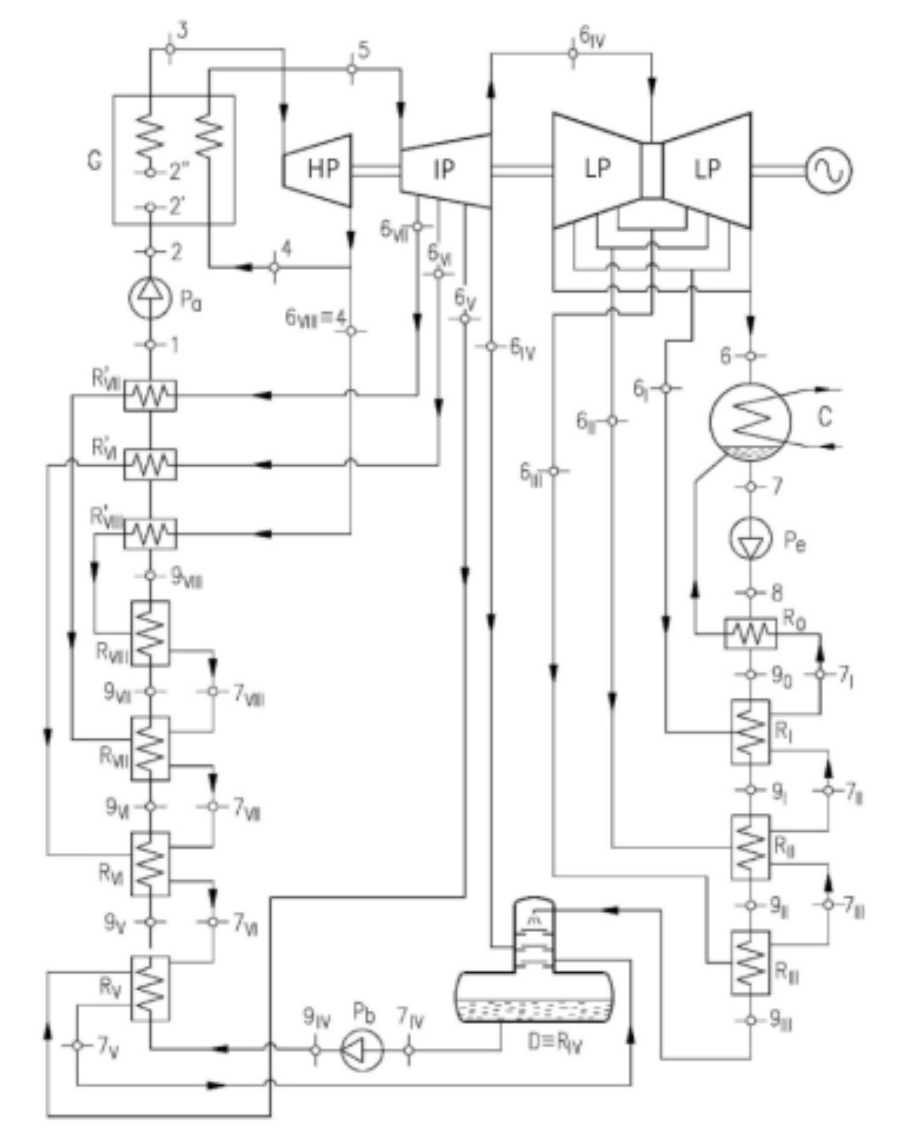
\includegraphics[width = 3.5in]{Figures/ST.png}
    \end{figure}
    
    \vfill

    \textbf{Authors:} \\
    Franklin Grégoire \\
    Hugo Warscotte

    \vspace{1cm}

    \textbf{Date of Submission:} \\
    \today

    \vspace{1cm}
    
    \textbf{Ecole Polytechnique de Louvain}

\end{titlepage}

\section*{Introduction}
As part of the \texttt{Thermal cycles} course, we were asked to model an advanced steam turbine cycle. 
This report first presents the main assumptions and methodology used, 
then presents the results obtained in default operating conditions.
Finally, a parametric analysis is performed to explore potential cycle improvements and efficiency gains.

\setcounter{section}{0} % Start numbering sections from 1
\section{General methodology and assumptions}
\subsection{Model assumptions}

The \textbf{main} assumptions used to model the steam turbine cycle are the following :
\begin{itemize}
    \setlength\itemsep{0em}
    \item The combustion process is modelled as a simple adiabatic heat transfer.
    \item The pressure losses in the steam generator are taken into account.
    \item Isobaric condensation.
    \item Adiabatic expansions in the turbines (the isentropic model is used).
    \item The pumps are electrically powered rather than mechanically driven by the same shaft as the turbines.
    \item For the exergy analysis, the expansion valves between each feedwater heater are neglected.
\end{itemize}

\subsection{Methodology}

In order to develop the model, we first computed the thermodynamic quantities for all states of the cycle.
Based on these quantities, we calculated the different flow rates
in the bleedings through energy balances at each feedwater heater.
The total flow rate of the cycle was determined using the power rating.
Finally, the energy and exergy losses were calculated using energy and 
exergy balances on each component of the cycle,
and the energetic and exergetic efficiencies were determined.


\section{Default conditions results}
In this section, we will review the results obtained with the model under default conditions. Those conditions are synthesized hereafter :

\begin{multicols}{3}
    \begin{itemize}
        \setlength\itemsep{0em}
        \item $P_e = 288 MW$
        \item $\eta_{pump} = 0.85$
        \item $\eta_{mec} = 0.98$
        \item $\eta_{is\_LP} = 0.90$
        \item $\eta_{is\_IP} = 0.90$
        \item $\eta_{is\_HP} = 0.92$
        \item $T_{drum} = 421.85K$
        \item $T_{max} = 838.15K$
        \item $T_{cd\_out} = 305.15K$
        \item $T_{cd\_subcool} = 1K$
        \item $p_3 = 31 MPa$
        \item $p_4 = 7 MPa$
    \end{itemize}
    \end{multicols}

\subsection{Table of the states obtained}


\begin{center}
\begin{longtable}{|c|c|c|c|c|c|c|}
    \hline
    States & $t \text{ } [^\circ C]$ & $p \text{ } [kPa]$ & $x \text{ } [-]$ & $h \text{ } [kJ/kg]$ & $s \text{ } [kJ/kgK]$ & $e \text{ } [kJ/kg]$\\
    \hline
    \endhead
    \hline
    \endfoot
    $1$ & $285.8$ & $10000$ & - & $1265.6$ & $3.112$ & $370.6$ \\
    $2$ & $293.5$ & $35000$ & - & $1295.1$ & $3.105$ & $401.9$ \\
    $3$ & $565.0$ & $31000$ & - & $3320.7$ & $6.077$ & $1571.1$ \\
    $4$ & $330.8$ & $7000$ & - & $2955.5$ & $6.130$ & $1190.6$ \\
    $5$ & $565.0$ & $6200$ & - & $3574.7$ & $7.056$ & $1543.0$ \\
    $6_{VII}$ & $485.0$ & $3751$ & - & $3414.7$ & $7.080$ & $1376.2$ \\
    $6_{VI}$ & $404.0$ & $2148$ & - & $3254.7$ & $7.106$ & $1208.6$ \\
    $6_{V}$ & $321.8$ & $1147$ & - & $3094.7$ & $7.136$ & $1039.9$ \\
    $6_{IV}$ & $238.4$ & $558$ & - & $2934.6$ & $7.172$ & $869.7$ \\
    $6_{III}$ & $154.1$ & $239$ & - & $2774.6$ & $7.214$ & $697.6$ \\
    $6_{II}$ & $95.6$ & $86$ & $0.98$ & $2614.6$ & $7.262$ & $523.7$ \\
    $6_I$ & $66.8$ & $27$ & $0.93$ & $2454.6$ & $7.314$ & $348.6$ \\
    $6$ & $33.0$ & $5$ & $0.89$ & $2294.5$ & $7.521$ & $128.9$ \\
    $7$ & $32.0$ & $5$ & $0.00$ & $134.1$ & $0.464$ & $1.9$ \\
    $9_{VII}$ & $246.6$ & $10000$ & - & $1069.4$ & $2.748$ & $279.2$ \\
    $9_{VI}$ & $216.0$ & $10000$ & - & $927.8$ & $2.467$ & $218.5$ \\
    $9_V$ & $185.9$ & $10000$ & - & $793.6$ & $2.184$ & $165.9$ \\
    $9_{IV}$ & $149.9$ & $10000$ & - & $637.8$ & $1.831$ & $111.9$ \\
    $7_{IV}$ & $148.7$ & $460$ & $0.00$ & $626.6$ & $1.829$ & $101.3$ \\
    $9_{III}$ & $125.9$ & $460$ & - & $529.1$ & $1.591$ & $72.2$ \\
    $9_{II}$ & $95.6$ & $460$ & - & $400.7$ & $1.257$ & $40.3$ \\
    $9_I$ & $66.8$ & $460$ & - & $279.9$ & $0.915$ & $17.8$ \\
    $8$ & $32.0$ & $460$ & - & $134.6$ & $0.464$ & $2.4$ \\
\end{longtable}
\end{center}

\vspace*{-1cm}

\subsection{T-s and h-s diagrams}
The T-s and h-s diagrams in default operating conditions are shown in figures \ref{fig:Ts_diagram} and \ref{fig:hs_diagram} respectively.
    
\begin{figure}[H]
    \centering
    % First figure
    \begin{minipage}{0.48\textwidth}
        \centering
        
\includegraphics[width=0.9\textwidth]{Figures/Ts_diagram.png}
        \caption{T-s diagram}
        \label{fig:Ts_diagram}
    \end{minipage}
    \hfill
    % Second figure
    \begin{minipage}{0.48\textwidth}
        \centering
        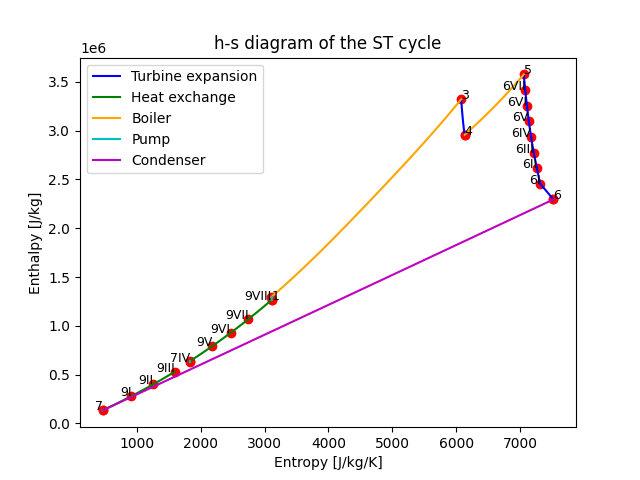
\includegraphics[width=0.9\textwidth]{Figures/hs_diagram.png}
        \caption{h-s diagram}
        \label{fig:hs_diagram}
    \end{minipage}
\end{figure}


\subsection{Energy and exergy pie charts}

The energy and exergy pie charts in default operating conditions are shown in figures \ref{fig:energy_pie_chart} and \ref{fig:exergy_pie_chart} respectively.

\begin{figure}[H]
    \centering
    % First figure
    \begin{minipage}{0.45\textwidth}
        \centering
        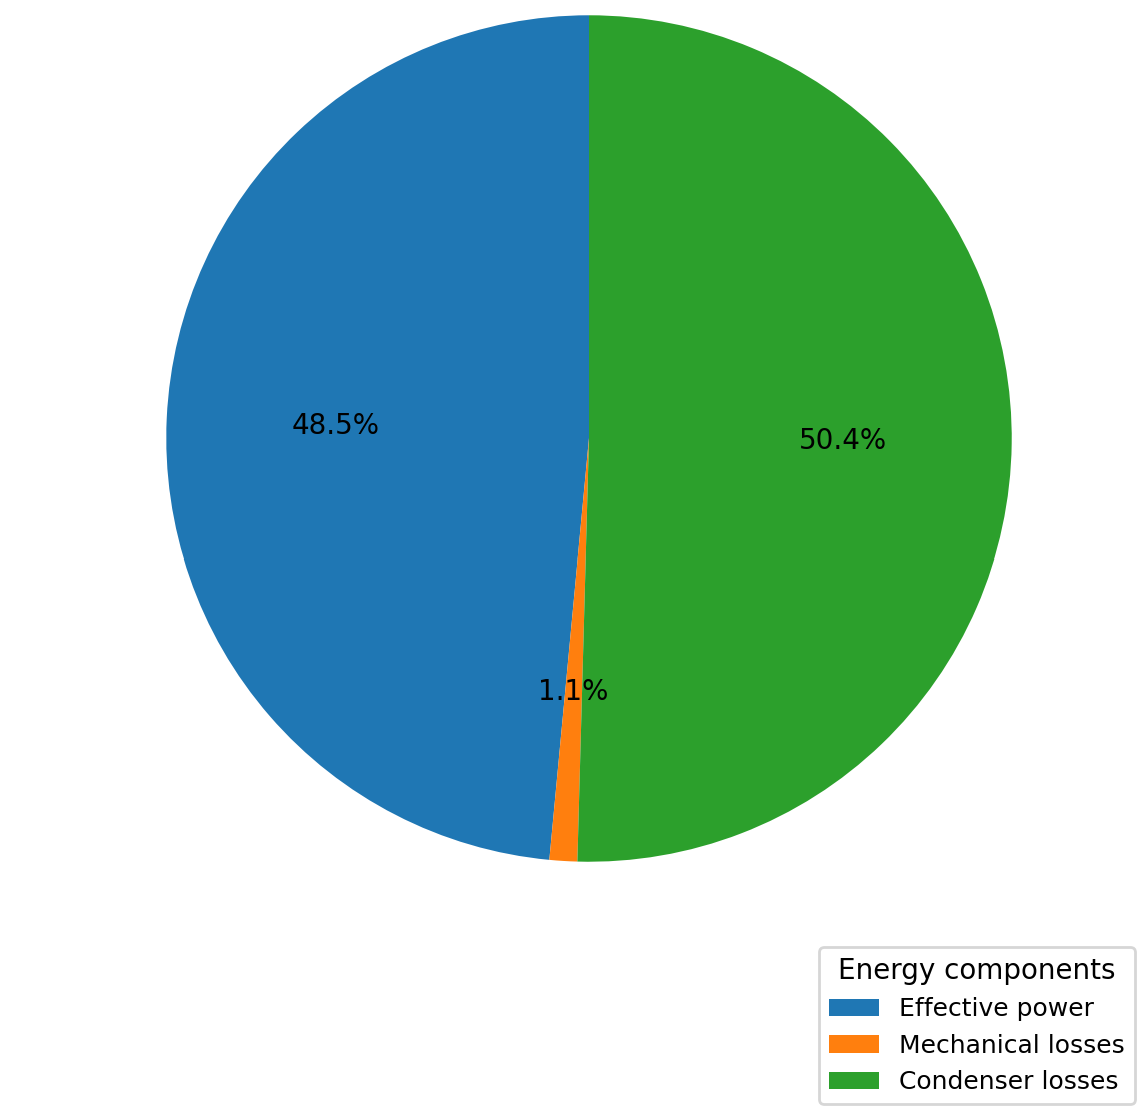
\includegraphics[width=0.7\textwidth]{Figures/pie_energy.png}
        \caption{Energy pie chart}
        \label{fig:energy_pie_chart}
    \end{minipage}
    \hfill
    % Second figure
    \begin{minipage}{0.43\textwidth}
        \centering
        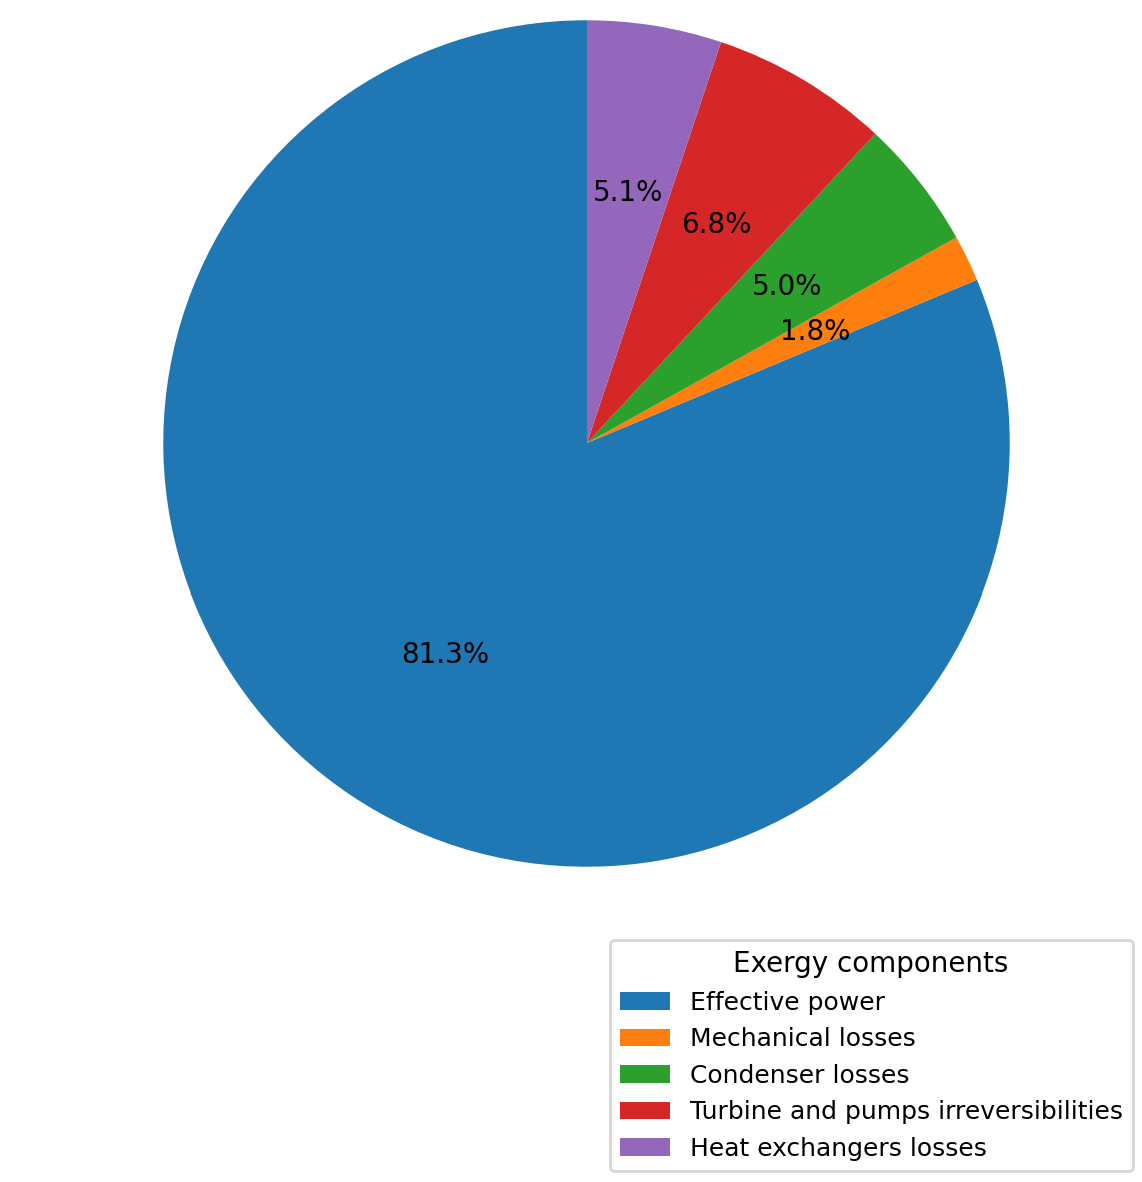
\includegraphics[width=0.7\textwidth]{Figures/pie_exergy.png}
        \caption{Exergy pie chart}
        \label{fig:exergy_pie_chart}
    \end{minipage}
\end{figure}

\section{Parametric analyses}
In this section, we will analyze how several
model parameters affect the system's performance.
First, we will examine the effect of the number of bleedings.
Next, we will analyse the effect of the number of reheatings.
Finally, the effect of the pressure at the high-pressure turbine inlet
will be discussed.

\subsection{Influence of the number of bleedings}

To analyse the influence of the number of bleedings, we varied
the number of bleedings in the low-pressure turbine from $0$ to $5$.
With the number of bleedings in the intermediate-pressure and high-pressure turbines kept constant,
this adjustment allowed the total number of bleedings to range from $5$ to $10$.
Our results are presented in figure \ref{fig:bleedings_results}.

\begin{figure}[H]
    \centering
    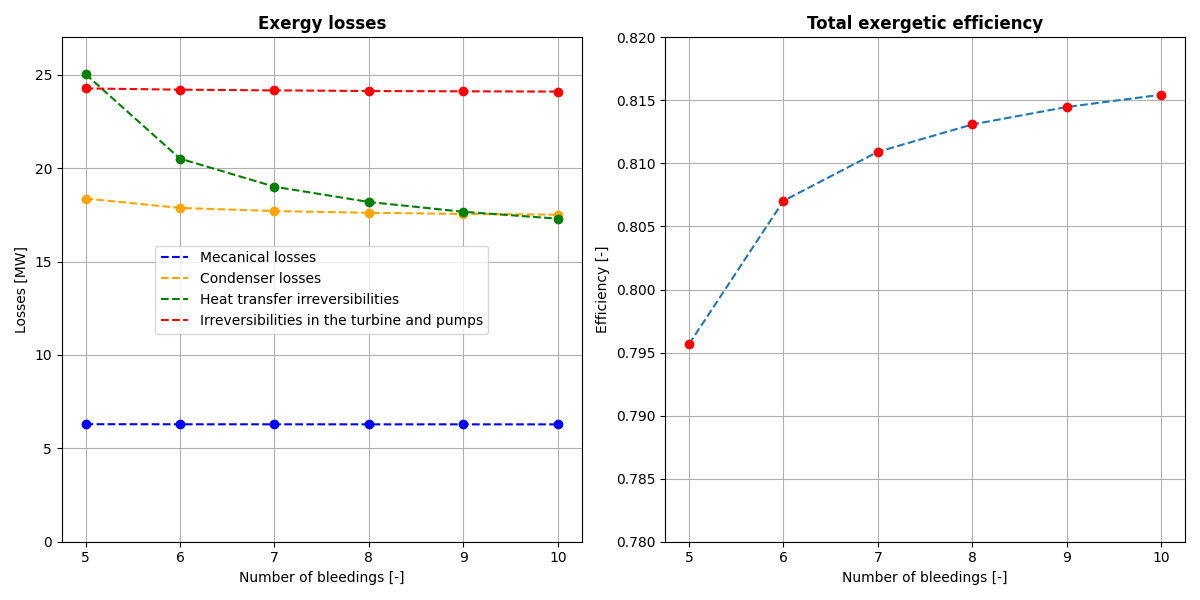
\includegraphics[width=0.5\textwidth]{Figures/bleedings.png}
    \caption{Influence of the number of bleedings on the system's performance.}
    \label{fig:bleedings_results}
\end{figure}

\noindent \textbf{Analysis :} As expected, the total exergetic efficiency 
increases with the number of bleedings but this increase is not linear and 
tends to saturate.  At one point, the costs related to the installation of 
an additional bleeding will exceed the benefits in terms of efficiency.
This benefit can be explained by three main factors :
\begin{enumerate}[noitemsep]
    \item When a bleeding is extracted from the turbine, the mass flow rate of steam 
    entering the condenser is reduced.  This reduces the exergy losses at the condenser ($p_{condex}$).
    \item The losses due to irreversibilities in the heat exchangers ($p_{transex}$) 
    are reduced because the extracted steam preheats the feedwater in stages, 
    lowering the temperature difference and minimizing exergy destruction.
    \item The mechanical losses ($p_{mec}$) and the losses due to irreversibilities in 
    the turbine and pumps ($p_{rotex}$) remain more or less constant.
\end{enumerate}
Consequently, as the number of bleedings increases, the overall exergy destruction in the cycle is reduced.\\


\noindent \textbf{Remark :} For this analysis, the total exergetic efficiency ($\eta_{totex}$)
is defined as follows ;
$$\eta_{totex} = \frac{P_e}{P_e + p_{transex} + p_{rotex} + p_{condex} + p_{mec}}$$
we obtain relatively high values ($\approx 80\%$) because the chimney losses, combustion
irreversibilities and heat transfer irreversibilities in the 
steam generator are not considered.



\subsection{Influence of the number of reheatings}
In this part, we will observe the influence of the number of reheating systems on the cycle. We will use the default conditions 
to compare the T-s diagrams of the cycle with zero reheating, one (see Fig. \ref{fig:Ts_diagram}) and two reheating systems.
The T-s diagrams of the zero reheating and two reheatings are shown in figures \ref{fig:0_reheating} and \ref{fig:2_reheatings} 
respectively.
First, we know, for the same conditions, that the zero reheating system won't be possible to implement. 
Indeed, the vapor quality at the low-pressure turbine outlet is inferior to the limit imposed by the Wilson line. Then, 
we will discuss over the two reheatings system. This cycle is as efficient as the default one (0.1 \% difference).
However, we can see that the vapor at the low-pressure turbine outlet is still overheated. Therefore, 
the mass flow rate of cooling fluid passing through the condenser is higher due to the higher enthalpy of the point 6.

\begin{figure}
    \begin{minipage}{0.48\textwidth}
       \centering
        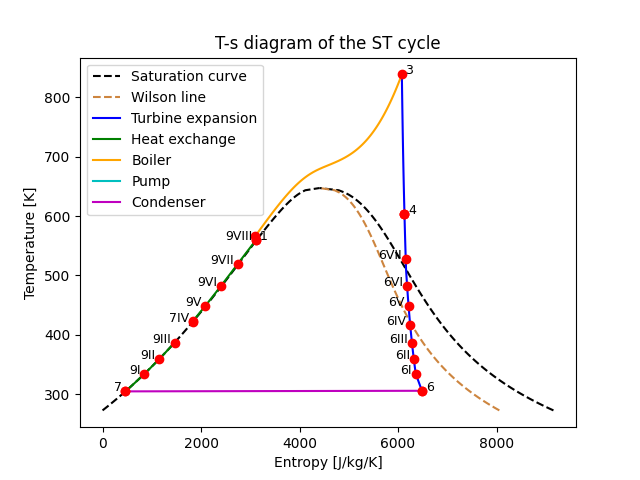
\includegraphics[width=0.75\textwidth]{Figures/ts_diagram_0_reheating.png}
        \caption{T-s diagram for zero reheating}
        \label{fig:0_reheating}    
    \end{minipage}
    \hfill
    \begin{minipage}{0.48\textwidth}
        \centering
        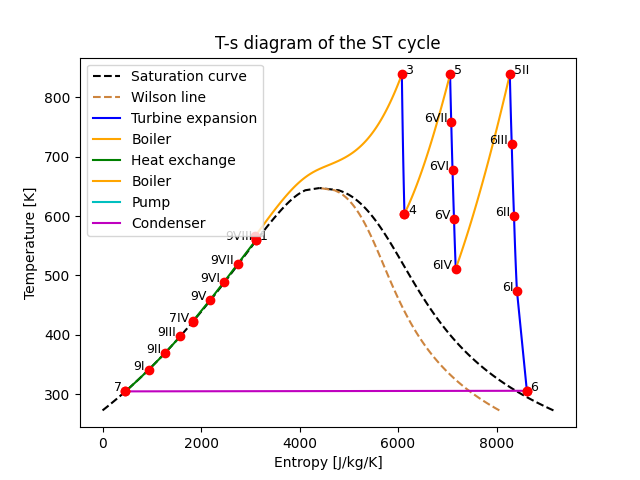
\includegraphics[width=0.75\textwidth]{Figures/ts_diagram_2_reheatings.png}
        \caption{T-s diagram for two reheatings}
        \label{fig:2_reheatings}
        
    \end{minipage}
\end{figure}





\subsection{Influence of the pressure at the high-pressure turbine inlet}
As final analysis, we will analyse the effect of the pressure at the high-pressure turbine inlet on the cycle.

\begin{figure}[h!]
    \begin{minipage}{0.48\textwidth}
       \centering
        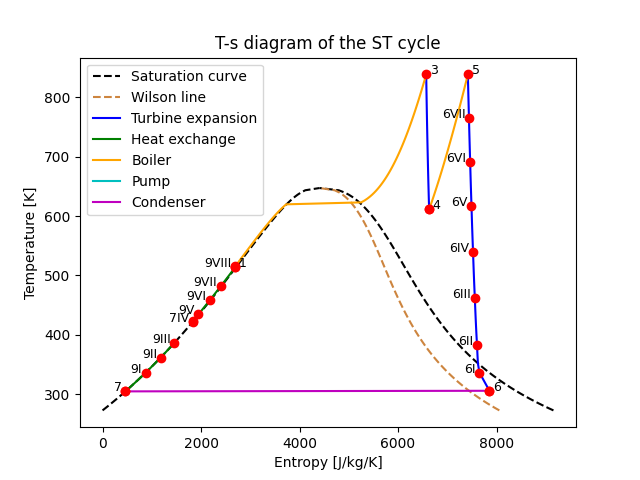
\includegraphics[width=0.75\textwidth]{Figures/ts_p_150.png}
        \caption{T-s diagram for $p_{3} = 15000$ kPa}
        \label{fig:p3_1}
        
    \end{minipage}
    \hfill
    \begin{minipage}{0.48\textwidth}
        \centering
        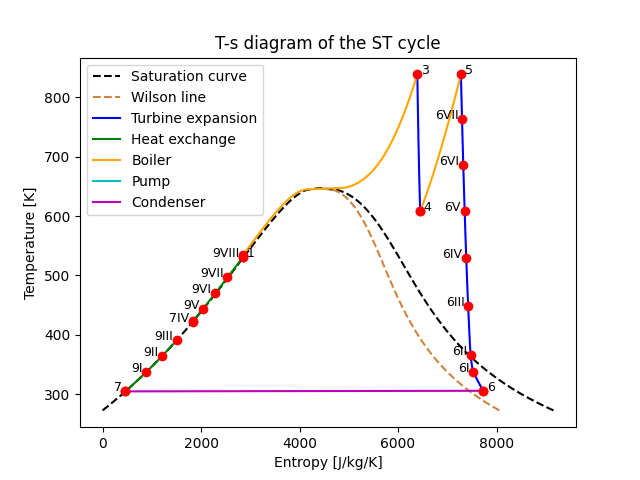
\includegraphics[width=0.75\textwidth]{Figures/ts_p_200.png}
        \caption{T-s diagram for $p_{3} = 20000$ kPa}
        \label{fig:p3_2}
    \end{minipage}
\end{figure}

We can see in figure \ref{fig:p3_1} that the pressure $p_3$ is under critical since we have a two-phase mixture in the boiler. 
In figure \ref{fig:p3_2}, the pressure is near the critical point. In the energy analysis, we can show that by increasing the pressure,
we increase the energy efficiency of the cycle (and the exergy efficiency). As $p_3$ increases from 15,000 kPa to 31,000 kPa, 
the total energy efficiency rises from 0.461 to 0.485. By using the supercritical cycle, the boiler doesn't 
need to provide latent heat to water. The drawback is that the infrastructure cost is higher (pump, materials, etc.).

\section*{Conclusion}
As conclusion, we can say that the numbers of bleedings and reheatings have a significant impact on the cycle's efficiency.
These numbers can vary depending on the application and the constraints. We also see that the Rankine cycle can be improved 
by using supercritical pressures. Compared to a gas power plant, the efficiency is higher but the constraints are more important.
Indeed, we need a source of cooling fluid and so, another cycle designed to manage the heat discharged by the condenser. Even though the 
Rankine cycle has been used for a long time with non-renewable sources, it can still be used in more modern applications. We can think
of combined cycle power plants or ROC's (Rankine Organic Cycles) which create electricity from heat waste or renewable sources.

\end{document}
